\subsection{Rancangan Detail Persistent Store}
\label{subsection:detail-persistent-store}

Komponen \textit{Persistent Store} bertanggung jawab untuk menyimpan data secara permanen. Komponen ini akan menggunakan sistem penyimpanan yang sesuai untuk memastikan bahwa data dapat disimpan dan diambil. Sesuai dengan bagian \ref{subsubsection:persistent-database}, komponen ini menggunakan RocksDB sebagai basis data penyimpanan. Rancangan komponen dapat dilihat pada gambar \ref{fig:persistent-store-component}.

\begin{figure}[ht]
    \centering
    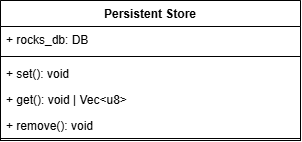
\includegraphics[width=0.4\textwidth]{resources/chapter-3/persistent-store-component.png}
    \caption{Struktur Komponen Komunikasi Antar-Node}
    \label{fig:persistent-store-component}
\end{figure}